% Joshua Reed
% Fall, 2017
% 
% hw1.tex
% 
% Homework for random processes.

% chktex-file 1 chktex-file 13 chktex-file 25 chktex-file 3 chktex-file 36

\documentclass[12pt]{article}
\usepackage[margin=1in]{geometry} 
\usepackage{amsmath,amsthm,amssymb}
\usepackage{listings}
\usepackage[compact]{titlesec}
\usepackage{graphicx}
\graphicspath{{img/}}

\setlength\parindent{00pt}
\setlength{\parskip}{\baselineskip}
\titlespacing{\section}{0pt}{5pt}{-\parskip}
\titlespacing{\subsection}{0pt}{-5pt}{-\parskip}
\titlespacing{\subsubsection}{0pt}{-8pt}{-\parskip}


\makeatletter
\renewcommand{\@seccntformat}[1]{}
\makeatother

% For Align:
%'*' tells LaTeX not to number lines.
%Align is a math environment. Thus \text{} is used for text contained within.
%'&' indicates a seperation between columns.

\begin{document}

{%Header section
  \large \bfseries 
  Joshua Reed

  Fall, 2017

  \begin{center}
    {\huge Homework 1}

    EE 520 - Random Processes \\% chktex 8 
  \normalsize Problems: 2.3, 2.7, 2.9, 2.10, 2.19, 2.22, 2.28, 2.30, 2.31, and 2.38
  \end{center}}
 
 
\section{2.3} 
\subsection{Exercise}
In a restaurant known for its unusual service, the time X, in minutes, that a customer has to wait
before he captures the attention of a waiter is specified by the following.

\begin{equation*}
  F_X(x)=\
    \begin{cases}
      (\frac{x}{2})^2, & \text{for }0\leq x \leq1,\\
      \frac{x}{4}, & \text{for }1\leq x \leq2,\\
      \frac{1}{2}, & \text{for }2\leq x \leq10,\\
      \frac{x}{20}, & \text{for }10\leq x \leq20,\\
      1, & \text{for }x\geq 20,
    \end{cases}
\end{equation*}

\subsubsection{Part A}
Sketch $F_x(x)$.
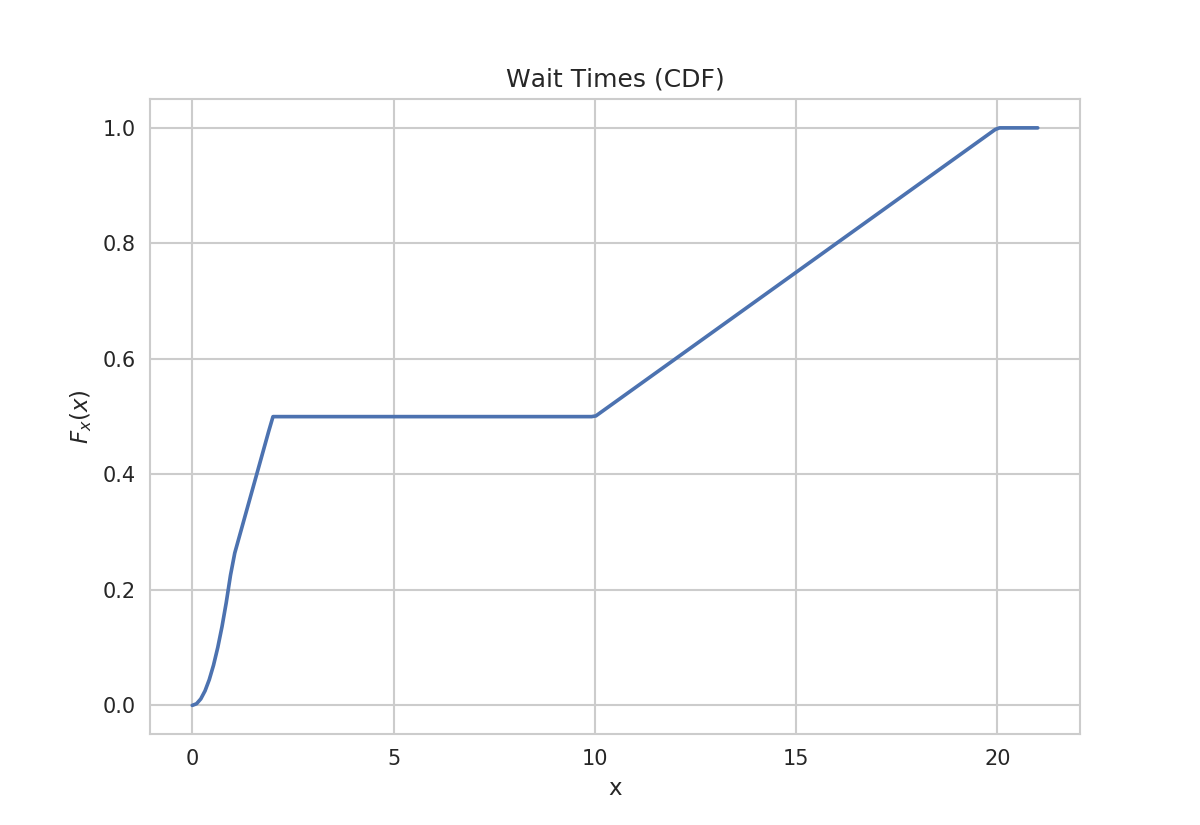
\includegraphics[scale=0.7]{plot-wait-times-cdf}

\subsubsection{Part B}
Compute and sketch the PDF $f_x(x)$

The PDF is the differential of the CDF, so the derivative of $F_x(X)$ will be the PDF $f_x(x)$.

For this problem, I am assuming that $F_x(x)$ is piecewise differentiable.\\
\begin{align*}
\frac{d}{dx}((\frac{x}{2})^2) &= \frac{d}{dx}(\frac{x^2}{4})\\
&= 2\frac{x}{4}\\
&= \frac{x}{2}
\end{align*}

\begin{align*}
\frac{d}{dx}(\frac{x}{4}) &= \frac{1}{4}
\end{align*}

\begin{align*}
\frac{d}{dx}(\frac{1}{2}) &= 0
\end{align*}

\begin{align*}
\frac{d}{dx}(\frac{x}{20}) &= \frac{1}{20}
\end{align*}

\begin{equation*}
  F_X(x)=\
    \begin{cases}
      \frac{x}{2}, & \text{for }0\leq x \leq1,\\
      \frac{1}{4},  & \text{for }1\leq x \leq2,\\
      0,            & \text{for }2\leq x \leq10,\\
      \frac{1}{20}, & \text{for }10\leq x \leq20,\\
      0,            & \text{for }x\geq 20,
    \end{cases}
\end{equation*}

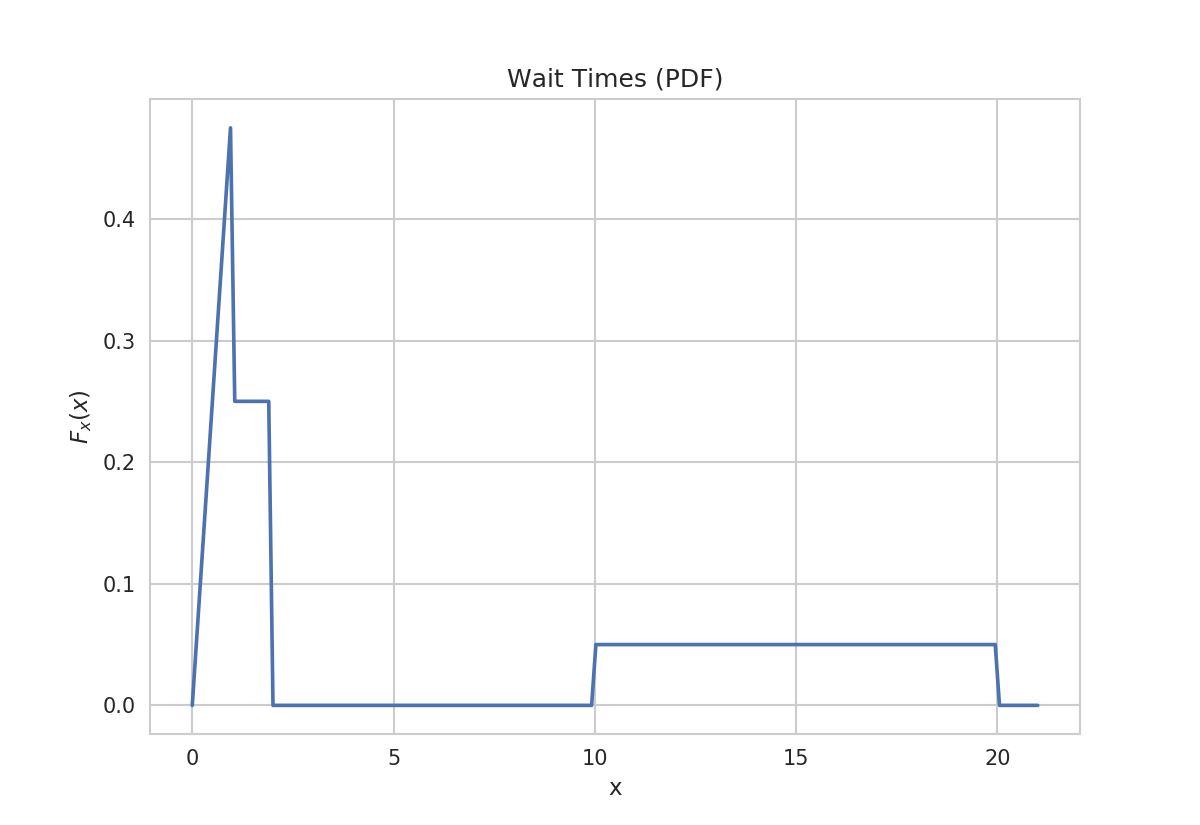
\includegraphics[scale=0.7]{plot-wait-times-pdf}

\subsubsection{Part C}
What is the probability that the customer will have to wait (1) at least 10 minutes, (2) less than 5 minutes, (3) between
5 and 10 minutes, (4) exactly 1 minute?

\begin{enumerate}
\item $P(X\geq10)=P(x\leq \infty)-P(x\leq10)=F_x(20)-F_x(10)=1-1/2=1/2$
\item $P(X\leq5)=F_x(5)=1/2$
\item $P(5\leq x \leq 10)=P(x\leq 10) -P(x\leq5)=1/2-1/2=0$
\item $P(x=1)=f_x(1)=$ either 1/2, 1/4, or more plausably 0.
\end{enumerate}

Because the likelihood of being served at {\bfseries exactly} 1 minute is zero.


\section{2.7} 
\subsection{Exercise}
A noisy resistor produces a voltage $v_n(t)$. At $t=t_1$, the noise level $X\stackrel{\Delta}{=}v_n(t_1)$ is known to be 
a Gaussian RV with PDF\\
\begin{align*}
f_X(x)=\frac{1}{\sqrt{2\pi\sigma^2}}e^{-\frac{1}{2}(\frac{x}{\sigma})^2}
\end{align*}
Compute and plot the probability that $|X|>k\sigma$ for $k=1,2,\ldots$






\section{2.9}
\subsection{Exercise}
Write PDFs using the $\delta$ functions for the Bernoulli binomial, and Poisson PMF's.
\subsection{Solution}
\subsubsection{Bernoulli PMF}
With probability of success p.
\begin{equation*} f_x(x)=
  \begin{cases}
    p^x(1-p)^{1-x},  & \text{for } x=0, 1 \\
    0, & \text{for all others}
  \end{cases}
\end{equation*}





\section{2.10}

\subsection{Exercise}
T pdf of a RV X is shown in figure P2.10. The numbers in the parenthesis indicate area. 
\subsection{Part A}
Compute the value of A.
\subsection{Part B}
Sketch the CDF.
\subsection{Part C}
Compute $P[2\leq X<3]$.
\subsection{Part D}
Compute $P[2<X\leq 3]$
\subsection{Part E}
Compute $F_x(3)$.

\section{2.19}
\subsection{Exercise}
It has been found that the number of people Y waiting in a queue in the bank on payday obeys the Poisson law as
\begin{align*}
P[Y=k|X=x]=e^{-x}\frac{x^k}{k!}, k\geq0, x>0
\end{align*}
given that the normalized serviing time of the teller x is constant. However, the serving time is more accurately modeled
as an RV X. For simplicity let X be a uniform RV with 
\begin{align*}
f_X(x)=\frac{1}{5}[u(x)-u(x-5)].
\end{align*}
Then $P[Y=k|X=x]$ is still Poisson but $P[Y=k]$ is something else. Compute $P[Y=k]$ for $k=1,2,$ and $2$. The answer for
general k may be difficult.

\section{2.22}
\subsection{Exercise}
Consider the joint PDF of X and Y:\\
\begin{align*}
f_{xy}(x,y)=\frac{1}{3\pi}e^{-\frac{1}{2}[(x/3)^2+(y/2)^2]}u(x)u(y)
\end{align*}
Are X and Y independent RVs? Compute the probability of $\{0<X\leq3, 0<Y\leq2\}$.


\section{2.28}
\subsection{Exercise}

\section{2.30}
\subsection{Exercise}

\section{2.31}
\subsection{Exercise}

\section{2.38}
\subsection{Exercise}



\end{document}
